% GHOST system model. Drawn at IEEE \textwidth (7.16in) so fonts render at true size.
\documentclass[tikz,border=1pt,10pt]{standalone}
\usepackage[T1]{fontenc}
\usepackage{mathptmx}
\usetikzlibrary{arrows.meta,calc,shapes.geometric}
\definecolor{navy}{HTML}{011E4B}
\definecolor{gold}{HTML}{FAB001}
\definecolor{sky}{HTML}{87C6E9}
\definecolor{alert}{HTML}{EE1C23}
\tikzset{
  >={Stealth[length=2.2mm,width=1.7mm]},
  font=\footnotesize,
  blk/.style={draw=navy,line width=0.6pt,fill=white,rounded corners=1.5pt,align=center,
              minimum height=10.5mm,text width=#1,inner sep=2pt,text=navy},
  blk/.default=15mm,
  db/.style={cylinder,shape border rotate=90,aspect=0.2,draw=navy,line width=0.6pt,
             fill=#1,align=center,text width=15mm,minimum height=8mm,inner sep=1pt,text=navy},
  db/.default=white,
  zone/.style={draw=#1,line width=1.1pt,rounded corners=3pt},
  head/.style={fill=#1,text=white,font=\footnotesize\bfseries,anchor=north west,
               inner xsep=4pt,inner ysep=2.5pt,rounded corners=1.5pt},
  f/.style={->,draw=navy,line width=0.8pt},
  fo/.style={->,draw=navy,line width=0.8pt,dash pattern=on 3pt off 2pt},
  n/.style={circle,fill=navy,text=white,font=\scriptsize\bfseries,inner sep=0pt,minimum size=4mm},
  lab/.style={font=\scriptsize,text=navy,inner sep=1.5pt},
}
\begin{document}
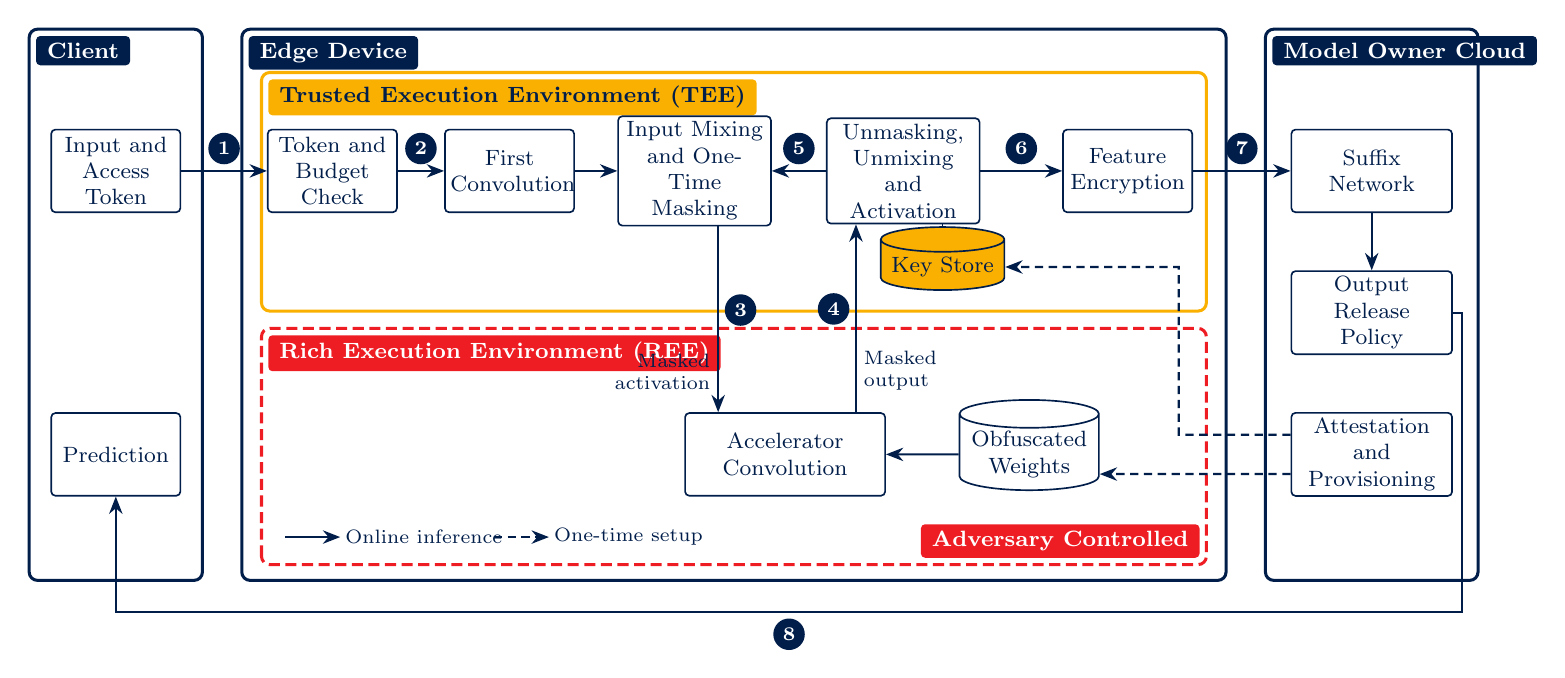
\begin{tikzpicture}
% ------------------------------------------------------------- zones
\draw[zone=navy] (0,0) rectangle (2.2,7.0);
\node[head=navy] at (0.08,6.92) {Client};
\draw[zone=navy] (2.7,0) rectangle (15.2,7.0);
\node[head=navy] at (2.78,6.92) {Edge Device};
\draw[zone=gold] (2.95,3.42) rectangle (14.95,6.45);
\node[head=gold,text=navy] at (3.03,6.37) {Trusted Execution Environment (TEE)};
\draw[zone=alert,dash pattern=on 4pt off 2pt] (2.95,0.2) rectangle (14.95,3.2);
\node[head=alert] at (3.03,3.12) {Rich Execution Environment (REE)};
\node[head=alert,anchor=south east] at (14.87,0.28) {Adversary Controlled};
\draw[zone=navy] (15.7,0) rectangle (18.4,7.0);
\node[head=navy] at (15.78,6.92) {Model Owner Cloud};

% ------------------------------------------------------------- blocks
\node[blk] (in)   at (1.1,5.2)  {Input and\\ Access Token};
\node[blk] (out)  at (1.1,1.6)  {Prediction};

\node[blk] (acl)  at (3.85,5.2)  {Token and\\ Budget\\ Check};
\node[blk] (c1)   at (6.1,5.2)  {First\\ Convolution};
\node[blk=18mm] (mask) at (8.45,5.2)  {Input Mixing\\ and One-Time\\ Masking};
\node[blk=18mm] (rec)  at (11.1,5.2) {Unmasking,\\ Unmixing and\\ Activation};
\node[blk] (enc)  at (13.95,5.2){Feature\\ Encryption};
\node[db=gold] (keys) at (11.6,3.98) {Key Store};

\node[blk=24mm] (acc) at (9.6,1.6) {Accelerator\\ Convolution};
\node[db,text width=17mm] (wst) at (12.7,1.6) {Obfuscated\\ Weights};

\node[blk=19mm] (suf)  at (17.05,5.2) {Suffix\\ Network};
\node[blk=19mm] (pol)  at (17.05,3.4) {Output Release\\ Policy};
\node[blk=19mm] (prov) at (17.05,1.6) {Attestation and\\ Provisioning};

% ------------------------------------------------------------- legend
\draw[f] (3.25,0.55) -- ++(0.7,0) node[right,lab]{Online inference};
\draw[fo] (5.9,0.55) -- ++(0.7,0) node[right,lab]{One-time setup};

% ------------------------------------------------------------- one-time setup
\draw[fo] ($(prov.west)+(0,0.25)$) -- (14.6,1.85) |- (keys.east);
\draw[fo] ($(prov.west)+(0,-0.25)$) -- ($(wst.east)+(0,-0.25)$);
\draw[navy,line width=0.6pt] (keys.north) -- (keys.north|-rec.south);

% ------------------------------------------------------------- online inference
\draw[f] (in) -- node[n,above=2pt]{1} (acl);
\draw[f] (acl) -- node[n,above=2pt]{2} (c1);
\draw[f] (c1) -- (mask);
\draw[f] (8.75,0|-mask.south) -- node[pos=0.45,n,right=2pt]{3} node[pos=0.78,lab,left=1pt,align=right]{Masked\\ activation} (8.75,0|-acc.north);
\draw[f] (10.5,0|-acc.north) -- node[pos=0.55,n,left=2pt]{4} node[pos=0.22,lab,right=1pt,align=left]{Masked\\ output} (10.5,0|-rec.south);
\draw[f] (wst) -- (acc);
\draw[f] (rec) -- node[n,above=2pt]{5} (mask);
\draw[f] (rec) -- node[n,above=2pt]{6} (enc);
\draw[f] (enc) -- node[n,above=2pt]{7} (suf);
\draw[f] (suf) -- (pol);
\draw[f] (pol.east) -- (18.2,0|-pol.east) -- (18.2,-0.4) -| node[pos=0.25,n,below=2pt]{8} (out.south);
\end{tikzpicture}
\end{document}
